%%%%%%%%%%%%%%%%%%%%%%%%%%%%%%%%%%%%%%%%%%%%%%%%%%%%%%%%%%%%%%%%%%%%
%% I, the copyright holder of this work, release this work into the
%% public domain. This applies worldwide. In some countries this may
%% not be legally possible; if so: I grant anyone the right to use
%% this work for any purpose, without any conditions, unless such
%% conditions are required by law.
%%%%%%%%%%%%%%%%%%%%%%%%%%%%%%%%%%%%%%%%%%%%%%%%%%%%%%%%%%%%%%%%%%%%

\documentclass{beamer}
\usetheme[logo=figures/McMasterLogo1,faculty=phil]{fibeamer}
\usepackage[utf8]{inputenc}
\usepackage[
  main=english, %% By using `czech` or `slovak` as the main locale
                %% instead of `english`, you can typeset the
                %% presentation in either Czech or Slovak,
                %% respectively.
  czech, slovak %% The additional keys allow foreign texts to be
]{babel}        %% typeset as follows:
%%
%%   \begin{otherlanguage}{czech}   ... \end{otherlanguage}
%%   \begin{otherlanguage}{slovak}  ... \end{otherlanguage}
%%
%% These macros specify information about the presentation
\title{\normalsize Instruction Scheduling} %% that will be typeset on the
\subtitle{Ph.D Candidate: Curtis D'Alves} %% title page.
\author{Supervisors: Dr. Wolfram Kahl, Dr. Christopher Anand}
%% These additional packages are used within the document:
\usepackage{ragged2e}  % `\justifying` text
\usepackage{booktabs}  % Tables
\usepackage{tabularx}
\usepackage{tikz}      % Diagrams
\usetikzlibrary{calc, shapes, backgrounds}
\usepackage{amsmath, amssymb}
\usepackage{url}       % `\url`s
\usepackage{listings}  % Code listings
\usepackage{float}
\usepackage{caption}
\usepackage{multicol}


\frenchspacing

\begin{document}
  \frame{\maketitle}

  \AtBeginSection[]{% Print an outline at the beginning of sections
    \begin{frame}<beamer>
      \frametitle{Table of Contents}
      \tableofcontents[currentsection]
    \end{frame}}

  \begin{darkframes}
%%%%%%%%%%%%%%%%%%%%%%%%%%%%%%%%%%%%%%%%%%%%%%%%%%%%%%%%%%%%%%%%%%%%%%%%%%%%%%%%%%%%%%%%%%%%%%%%%%%%%%%%%%%%%%%%
%%%%%%%%%%%%%%%%%%%%%%%%%%%%%%%%%%%%%%%%%%%%%%%%%%%%%%%%%%%%%%%%%%%%%%%%%%%%%%%%%%%%%%%%%%%%%%%%%%%%%%%%%%%%%%%%
%%%%%%%%%%%%%%%%%%%%%%%%%%%%%%%%%%%%%%%%%%%%%%%%%%%%%%%%%%%%%%%%%%%%%%%%%%%%%%%%%%%%%%%%%%%%%%%%%%%%%%%%%%%%%%%%
    \section{Introduction}
\begin{frame}{Instruction Scheduling}

	{\color{cyan} \bf Problem:} Given a set of instructions and dependencies, designate an order (find a {\it schedule}) satisfying the dependencies and optimizing performance
	\pause
	\qquad \\
	\qquad \\
	\qquad \\
	Known {\bf \color{green} NP-Complete} problem, practically solved by
	\begin{itemize}
		\item Heuristics
		\item Approximation Algorithms
	\end{itemize}
\end{frame}      

\begin{frame}[fragile]
  \frametitle{Example: Dependency Graph (DAG)}

  \begin{figure}
  \begin{lstlisting}
  load r1 0xFFFF
  load r2 0xFFF1
  load r3 0xFFF2                    (r1 + r2) * (r1 + r3)
  add r4 r2 r1
  add r5 r3 r1
  mult r6 r4 r5
  \end{lstlisting} 
    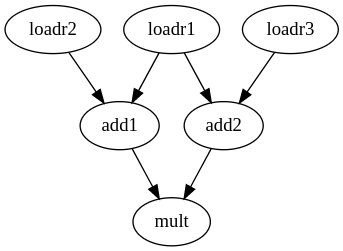
\includegraphics[scale=0.3]{figures/depgraph.png}
  \end{figure}
\end{frame}

\begin{frame}[fragile]
  \frametitle{Instruction Schedules}
\begin{lstlisting}
  load r1 0xFFFF      load r1 0xFFFF
  load r2 0xFFF1      load r2 0xFFF1
  load r3 0xFFF2      add r3 r2 r1
  add r4 r2 r1        load r2 0xFFF2
  add r5 r3 r1        add r4 r2 r1
  mult r6 r4 r5       mult r5 r4 r3
\end{lstlisting} 
  \begin{itemize}
  \item Both of the above orders (i.e schedules) are {\bf \color{green} valid} (i.e
  don't break dependencies)
  \item What's the difference:
  \begin{itemize}
    \item {\bf \color{cyan} peformance}
    \item {\bf \color{cyan} number of registers used}
  \end{itemize}
  \end{itemize}
\end{frame}

\begin{frame}[fragile]
  \frametitle{Complication: Branching}
  
\begin{lstlisting}
  load r1 0xFFFF
  load r2 0xFFF1
  load r3 0xFFF2 
  add r4 r2 r1 <---
  add r5 r3 r1    |
  mult r6 r4 r5   |
  branch 0x0003 ---
  add r2 r4 r1   
\end{lstlisting} 
  Control flow (like {\bf \color{green} loops} and {\bf \color{green}
    conditionals}) complicate scheduling
\end{frame}

\subsection{Types of Scheduling}
\begin{frame}{Types of Scheduling}

\begin{itemize}
	\item {\bf \color{green} Basic Block:} break code into blocks within branches {\bf \color{cyan} (most commonly performed scheduling)} \\
	\qquad \\
	\pause
	\item {\bf \color{green} Global Scheduling:} schedule across basic block boundaries \\
	\qquad \\
	\pause
	\item {\bf \color{green} Modulo Scheduling:} an algorithm to increase pipelining of loops by interleaving different iterations \\
	\qquad \\
	\pause
	\item {\bf \color{green} Trace Scheduling:} tries to optimize control flow by predicting routes taken on branches
\end{itemize}
\end{frame}

\begin{frame}{Modulo Scheduling: Staged Loop}
  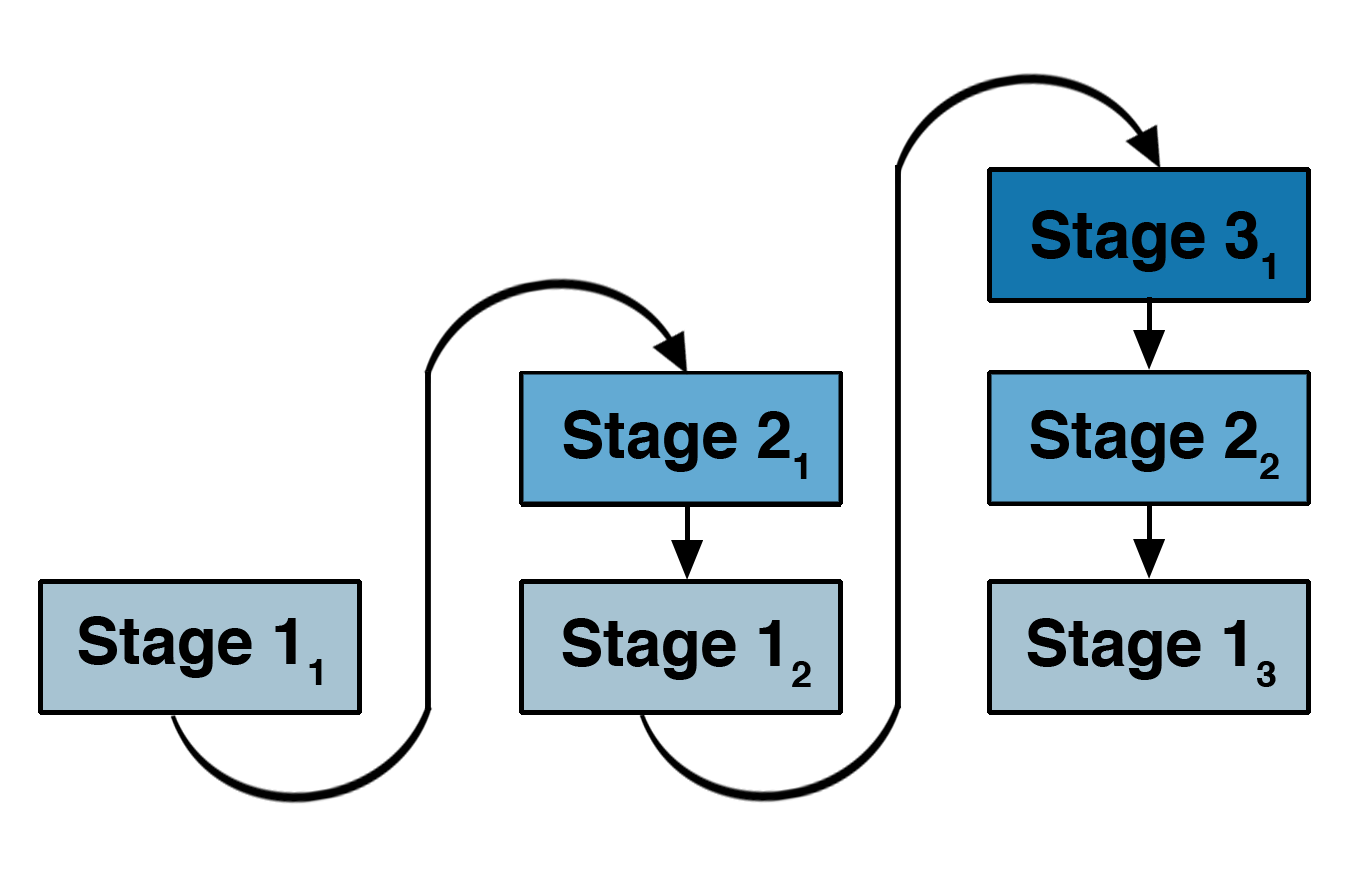
\includegraphics[scale=0.15]{figures/staging.png}

When performing {\bf \color{green} modulo scheduling}, a basic block of a loop can be broken
into stages and the loop can be {\bf \color{cyan} rolling} to interleave stages between
iterations
\end{frame}

% \subsection{Example Dependency DAG}
% \begin{frame}{Example: Instruction Dependency DAG}
% \begin{figure}
% 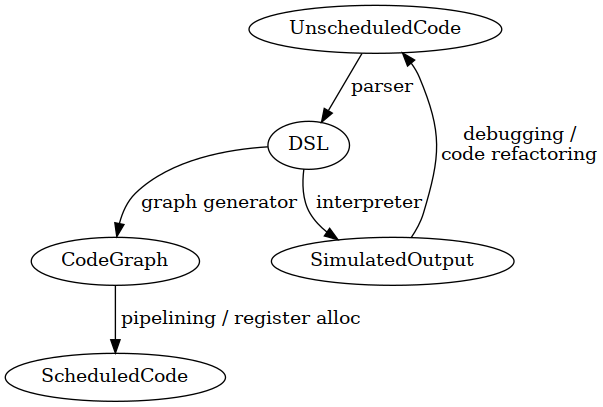
\includegraphics[scale=0.085]{figures/graph}
% \caption{Vector Instruction Dep. Graph}
% \end{figure}
% \end{frame}

\section{Pipelining}
\begin{frame}{Classic RISC Pipeline}
\begin{figure}
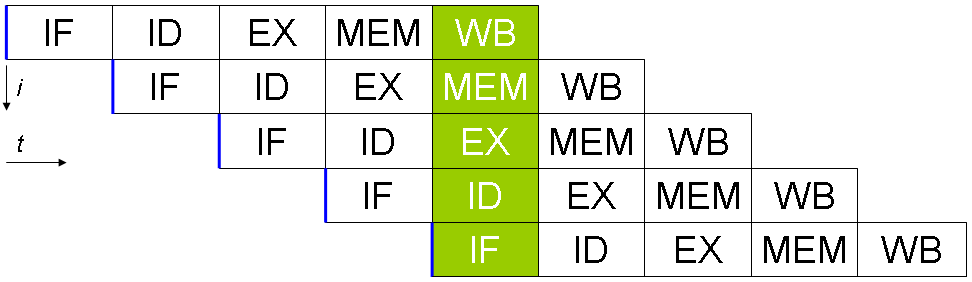
\includegraphics[scale=0.4]{figures/pipeline}
\caption{Example Pipeline}
\end{figure}
\end{frame}

\begin{frame}{SuperScaler Pipelining}
\begin{figure}
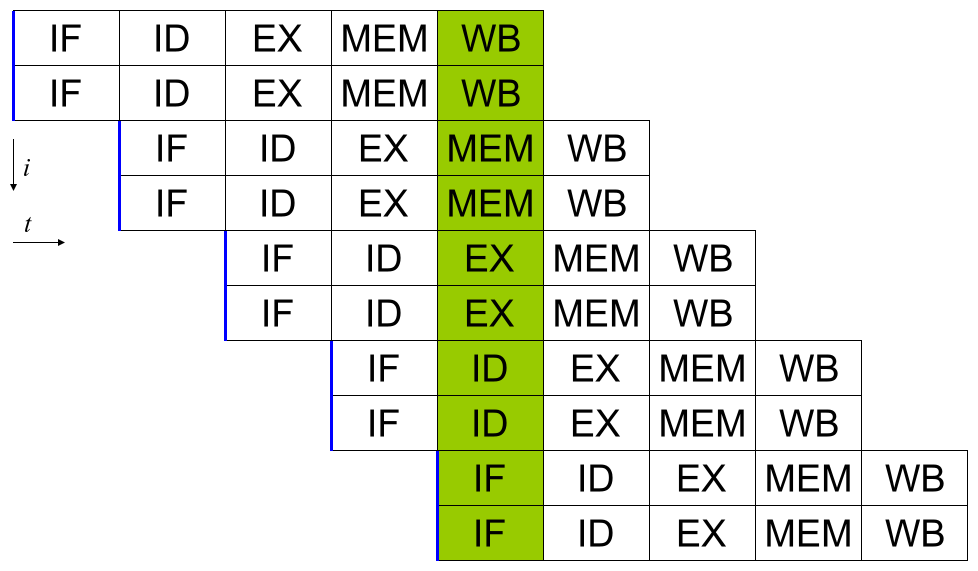
\includegraphics[scale=0.3]{figures/superscaler}
\caption{Example SuperScaler Pipeline}
\end{figure}
\end{frame}

\subsection{Out-of-order Execution}
\begin{frame}{Out-of-order Execution}
  \begin{figure}
    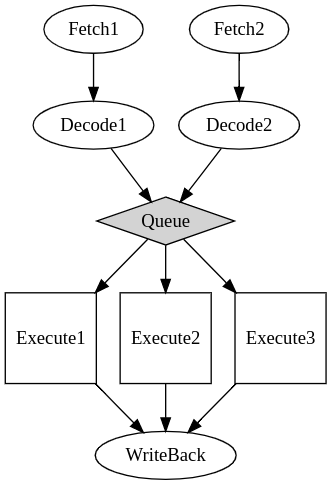
\includegraphics[scale=0.3]{figures/FunctionalUnits.png}
    \caption{Example SuperScaler Pipeline}
  \end{figure}
\end{frame}

\begin{frame}{Out-of-order Execution}
	\begin{enumerate}
  \item Instruction fetch
  \item Dispatch to instruction queue
  \item Instruction waits until its input is available, then allowed to leave queue (in whatever order)
  \item Instruction is executed
  \item Results are queued
  \item Only after all older instructions have their results written back to registers, the instruction's result is written back to registers 
	\end{enumerate}
\end{frame}

\subsection{Hazards}
\begin{frame}{Hazards}
	\begin{itemize}
		\item {\bf \color{green} Data Hazards}
		\begin{itemize}
			\item read after write {\color{cyan} (RAW)}
			\item write after read {\color{cyan} (WAR)}
			\item write after write {\color{cyan} (WAW)}
		\end{itemize}
		\qquad \\
		\qquad \\
		\pause
		\item {\bf \color{green}  Structural Hazards} - occurs when an aspect of hardware is accessed at the same time
		\qquad \\
		\qquad \\
		\pause
		\item {\bf \color{green} Control Hazards} - caused by branching, next instruction unknown
	\end{itemize}
\end{frame}

\subsection{Pipeline Stalls / Bubbles}
\begin{frame}{Pipeline Stalls / Bubbles}
\begin{figure}
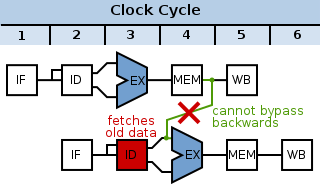
\includegraphics[scale=0.4]{figures/bubbles}
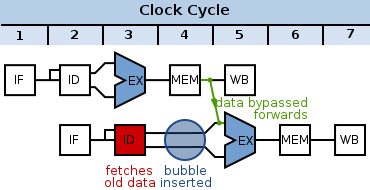
\includegraphics[scale=0.4]{figures/bubbles2}
\caption{Pipeline Stall}
\end{figure}

A {\bf \color{green} Ideal Schedule} contains NO bubbles (often not possible)
\end{frame}


\section{Register Allocation}

\begin{frame}{Register Allocation}

	{\bf \color{cyan} Problem:} Given a schedule, assign registers keeping in mind
	\begin{itemize}
		\item limited \# of registers
		\item can't rewrite a register until consumed by dependent instructions
	\end{itemize}
	\qquad \\
	\qquad \\
	Once again, known {\bf \color{green} NP-Complete} problem. Practically solved by using non-optimal {\bf \color{green} Graph Coloring} problems 
\end{frame}

\subsection{Graph Coloring}
\begin{frame}{Graph Coloring}
\begin{figure}
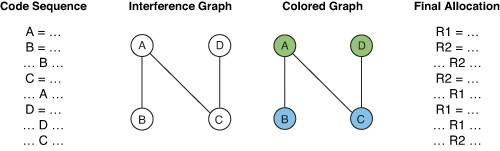
\includegraphics[scale=0.5]{figures/nshape}
\caption{Register Allocation via Graph Coloring}
\end{figure}
Find a {\bf \color{green} k-Coloring} for the interference graph, where {\bf \color{green} $k = \#\textsc{Registers}$}
\end{frame}

\subsection{Spilling}
\begin{frame}{Spilling}
	\begin{itemize}
		\item What if a {\bf \color{cyan} k-Coloring} can't be found? Must {\bf \color{green} Spill} memory \\
		\qquad \\
		\pause
		\item Simply insert new {\bf \color{cyan} Load / Store} instructions as needed \\
		\qquad \\
		\pause
		\item Potentially {\bf \color{cyan} creates new bubbles} in the pipeline, need to re-perform scheduling \\
		\qquad \\
		\pause
		\item An {\bf \color{cyan} Ideal Schedule} has no spilling 
	\end{itemize}
\end{frame}

\section{List Scheduling}
\begin{frame}{List Scheduling}
	Simple heuristic.  Choose a {\bf \color{cyan} prioritized topological order} that \\
	\qquad \\
	\begin{itemize}
		\item Respects the edges in the data-dependence graph ({\bf \color{green} topological}
		\item Heuristic choice among options, e.g pick first the node with the longest path extending from that node {\bf \color{green} prioritized}
	\end{itemize}
	\qquad \\
	\qquad \\
	Most commonly used method for scheduling. Efficient but yields far less than optimal schedules
\end{frame}

\begin{frame}{Issues with List Scheduling}

    \begin{itemize}
        \item Many factors to consider when constructing a schedule (everything listed in this presentation and more!) \\
        \qquad \\
        \pause
        \item Difficult (or more accurately impossible!) to consider all these aspects into a single choice heuristic \\
        \qquad \\
        \pause
        \item Combinations of heuristics can be used, and multiple iterations performed, but each will usually undo the work of the other
    \end{itemize}
\end{frame}

\section{My Research}
\begin{frame}{My Research}

    \begin{itemize}
        \item Scheduling of pre-compiled binaries \\
        \qquad \\
        \pause
        \item Since pre-compiled, my algorithm can afford to be {\bf \color{green} less efficient} and seek {\bf \color{green} near-optimal performance} \\
        \qquad \\
        \pause
        \item Uses a {\bf \color{green} Continuous Optimization Model}
    \end{itemize}
\end{frame}

\begin{frame}{Continuous Optimization}

  \begin{figure}
    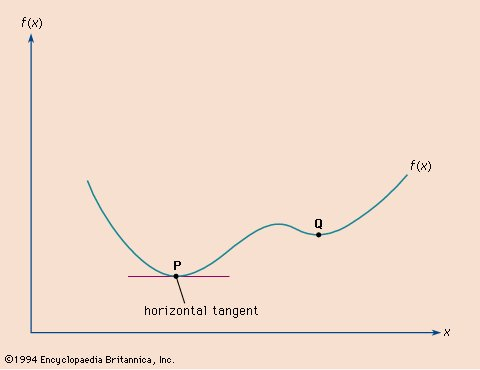
\includegraphics[scale=0.4]{figures/optimization.jpg}
    \caption{Ref https://www.britannica.com/topic/nonlinear-programming}
  \end{figure}
  Find a minumum of a funciton $f(x)$

\end{frame}

\begin{frame}{Relaxed Continuous Optimization based Scheduling}
    Per Instruction $i$, perform a relaxation of scheduled position to dispatch and completion times $t_i$,$b_i$
    \begin{align*}
    \text{\color{cyan} Objective Variables \qquad} & t_i, b_i, f_i:& \mathbb{R} \\
    \text{\color{cyan} Constants \qquad} & \textrm{II} :& \mathbb{R} \\
    \text{\color{cyan} Indicator Function \qquad} & \mathbb{IN} :& \mathbb{R} \rightarrow \mathbb{R} \\
    & t_i :& \text{dispatch time} \\
    & b_i :& \text{completion time} \\
    & f_i :& \text{FIFO use } 0 \leq f_i \leq 1 \\
    & \textrm{II} :& \text{iteration interval} \frac{\# instructions}{dispatches/cycle} \\
    \end{align*}
   
\end{frame}

\begin{frame}{Relaxed Continuous Optimization based Scheduling}
    \begin{align}
    \text{\color{cyan} Hard Constraints \qquad}  & t_i + \epsilon \leq t_j \qquad & \forall i,j \cdot i \rightarrow j \\
								 & 0 \leq t_i \leq b_i \leq \#\text{stages} \cdot \textrm{II}  & \\
								 & b_i + \epsilon \leq t_i + \textrm{II} \\
    \text{\color{cyan} Objective Function \qquad}   & \text{min} \sum_{i} (b_i - t_i + f_i) + \text{Penalties}
    \end{align}
    
    {\bf \color{green} Key Idea:} Encode choice heuristics as penalties, adjust preference by between heuristics scaling
\end{frame}

\begin{frame}{Relaxed Continuous Optimization based Scheduling}

    {\bf \color{green} Other Key Idea:} Need to construct penalty to prevent {\bf \color{cyan} Spilling}. Need to prevent clobbering of certain types of instructions \\
    {\bf \color{green} Solution:} Indicator function to detect penalize clobbering
    \begin{figure}
        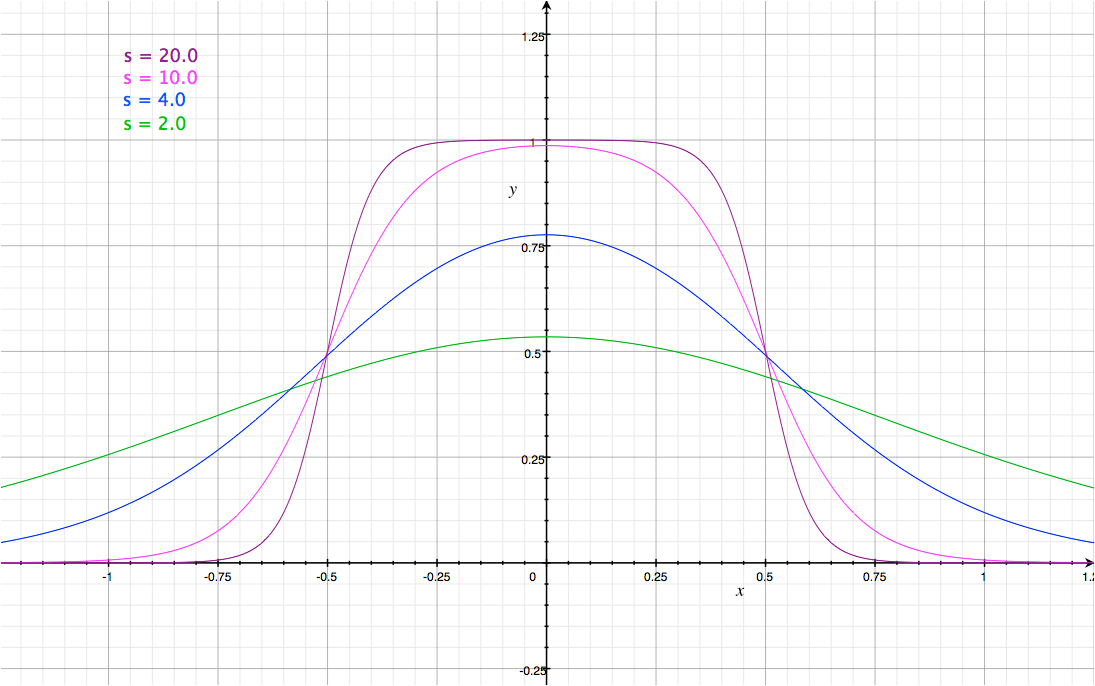
\includegraphics[scale=0.2]{figures/sigmoid}
        \caption{Altered Sigmoid Indicator Function}
    \end{figure}

\end{frame}

%%%%%%%%%%%%%%%%%%%%%%%%%%%%%%%%%%%%%%%%%%%%%%%%%%%%%%%%%%%%%%%%%%%%%%%%%%%%%%%%%%%%%%%%%%%%%%%%%%%%%%%%%%%%%%%%
%%%%%%%%%%%%%%%%%%%%%%%%%%%%%%%%%%%%%%%%%%%%%%%%%%%%%%%%%%%%%%%%%%%%%%%%%%%%%%%%%%%%%%%%%%%%%%%%%%%%%%%%%%%%%%%%
%%%%%%%%%%%%%%%%%%%%%%%%%%%%%%%%%%%%%%%%%%%%%%%%%%%%%%%%%%%%%%%%%%%%%%%%%%%%%%%%%%%%%%%%%%%%%%%%%%%%%%%%%%%%%%%%
    \section{Questions?}                           % Questions?
    \begin{frame}{Questions?}
    \end{frame}
    
  \end{darkframes}

\end{document}
